\chapter{Présentation des frameworks d'édition d'images (15 pages) }
	
	Dans ce mémoire nous discuterons d'un ensemble d'algorithmes constituant un framework
	de rendu et d'édition d'images nommé \emph{Himalaya}. Par le terme framework nous entendons une
	librairie présentant une interface logicielle permettant d'éditer des images. \index{Framework d'edition d'images} De tels frameworks sont
	ensuite utilisés par diverses applications, comme les logiciels de peinture, d'édition 3D, les jeux-vidéos,
	les logiciels de cartographie, les interfaces multimédia, etc. 
	
	Nous allons premièrement examiner quelles sont les fonctionalités requises aujourd'hui pour un tel framework 
	et ensuite examiner les manières les plus populaires de les implémenter, afin de voir où ce situe \emph{Himalaya}
	Dans le paysage des frameworks d'éditon d'images.

	\section{Cahier des charges pour un framework d'édition d'image}
		\subsection{Opérations de dessin}
			L'opération de base d'un framework d'édition d'image est bien évidemment de permettre de 
			modifier une image. On distingue plusieurs manières de le faire qui seront traitées différemment
			selon les implémentations.
			\subsubsection{Dessin de primitives}
				Par dessin de primitive on entend l'ajout sur l'image de primitives géométriques, comme
				des polygones, des lignes, des points, des cercles, du texte, etc. Ces primitives ont généralement un 
				effet local sur l'image, c'est à dire qu'elles ne la modifient pas dans son intégralité. On s'attend généralement
				de la part d'un framework d'édition d'image que de telles opérations soient peu couteuse en
				temps et en mémoire, étant donné que la réalisation d'un dessin intéressant nécessite généralement
				un nombre très élevé de primitives, jusqu'a plusieurs millions.
				\index{Primitives, dessin de}
				\begin{figure}[h]
					\centering
					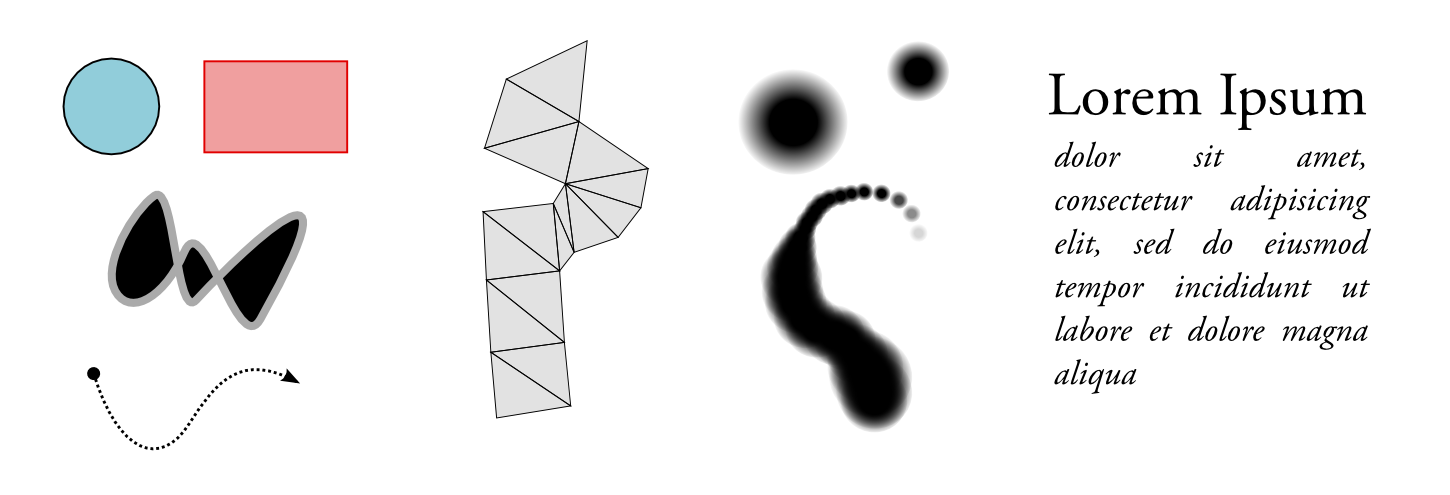
\includegraphics[width=\textwidth]{images/primitives}
					\caption{Examples de dessins de primitives}
					\label{fig:primitives}
				\end{figure}
			\subsubsection{Filtres}
				\index{Filtres}
				Un filtre est une opération qui modifie l'aspect de l'entièreté d'une image. De par leur nature
				les filtres peuvent être coûteux en temps, certains filtres fort complexes comme le \emph{Content Aware Fill}
				peuvent prendre plusieurs minutes à appliquer et ceci indépendemment du framework dans lequel ils
				sont utilisés. De par leur coût temporel, la réalisation d'un dessin n'utilise qu'un nombre réduits
				de filtres, dépassant rarement la centaine. 
				

				Les filtres peuvent être également partagés en deux catégories,\index{Filtres!colorimetriques} les filtres colorimétriques qui transforment
				la couleur d'un pixel sans se soucier de la couleur des pixels voisins, \index{Filtres!spatiaux} et les filtres spatiaux nécessitant 
				eux d'en connaître plusieurs. 
				\begin{figure}[h]
					\centering
					\subfloat[Image originale]{ \label{fig:lenna} 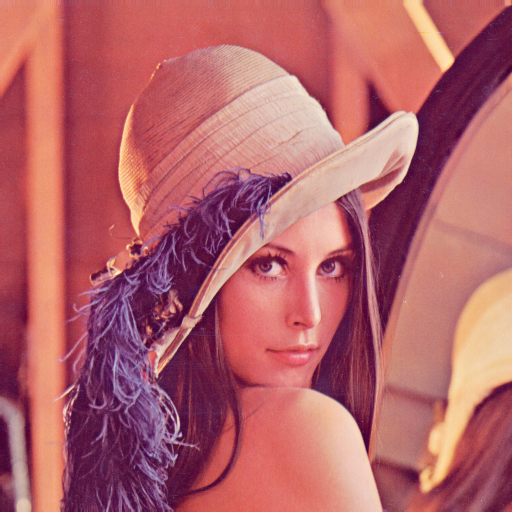
\includegraphics[width=0.3\textwidth]{images/Lenna} }
					\subfloat[Filtre colorimétrique]{ \label{fig:lenna} 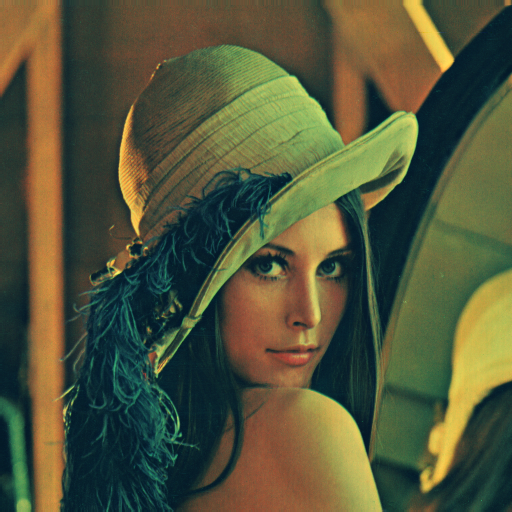
\includegraphics[width=0.3\textwidth]{images/Lenna-green} }
					\subfloat[Filtre spatial \emph{Sobel}]{ \label{fig:lenna} 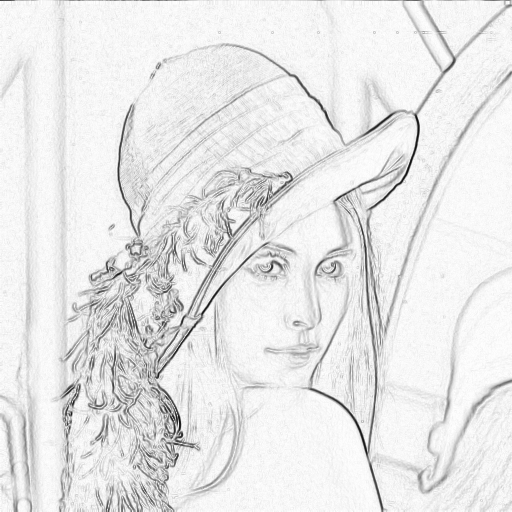
\includegraphics[width=0.3\textwidth]{images/Lenna-sobel} }
					\caption{Examples de filtres}
					\label{fig:filtres}
				\end{figure}
			\subsubsection{Transformations géométriques}
				Les transformations géométriques modifient la forme d'un objet constituant l'image; rotation, translation, 
				redimentionnement, perspective, mapping géométrique sont les applications les plus courantes. 
				
				L'efficacité des transformations géométriques varie très fortement d'une implémentation à l'autre. L'usage
				intensif de celles-ci est souvent un facteur déterminant dans le choix du framework.
			\subsubsection{Blending}
				Le blending consiste à fusionner plusieurs images en une en les superposant. Il existe un nombre très varié
				de manières d'interpréter la superpositon de deux images, la plus commune étant l'opacité : Pour un paramètre
				$\alpha \in [0,1]$ déterminant l'opacité de B, le résultat de la superposition de $A$ sur $B$ est 
				$\alpha * A +  (1-\alpha) * B$. Le blending est une opération centrale dans tout framework d'édition d'image.

				\begin{figure}[h]
					\centering
					\subfloat[Image A]{ \label{fig:A} 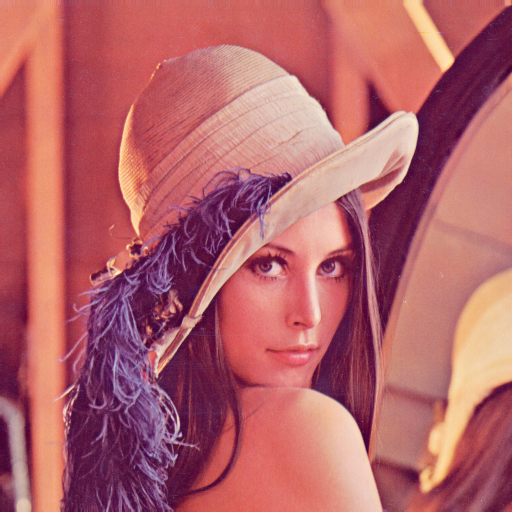
\includegraphics[width=0.25\textwidth]{images/Lenna} }
					\subfloat[Image B]{ \label{fig:B} 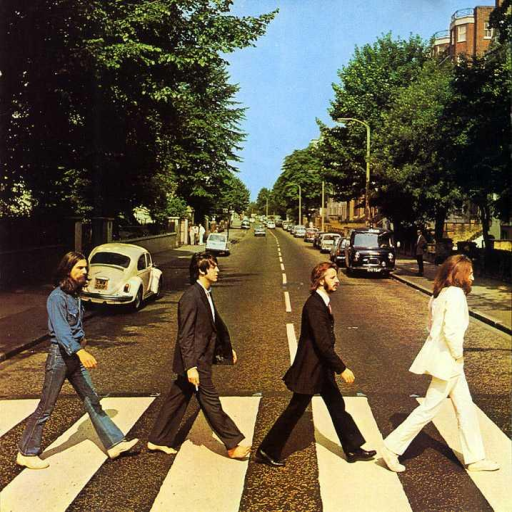
\includegraphics[width=0.25\textwidth]{images/abbey-road} }
					\subfloat[Blending de B sur A, par \emph{fusion de grain} ]{ \label{fig:ABfusion} 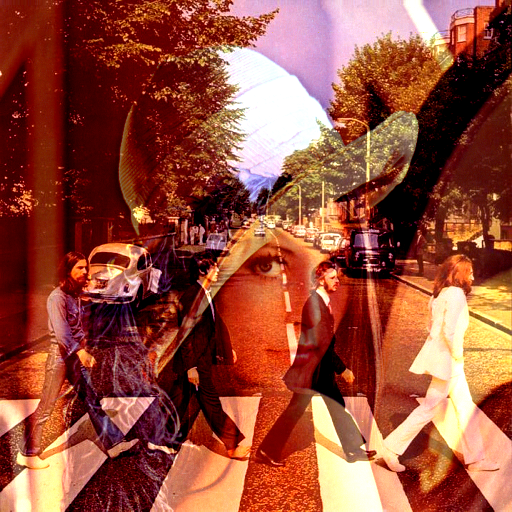
\includegraphics [width=0.25\textwidth]{images/abbey-road-lenna-fusion} }
					\subfloat[Blending de B sur A, par \emph{soustraction} ]{ \label{fig:ABsoustraction} 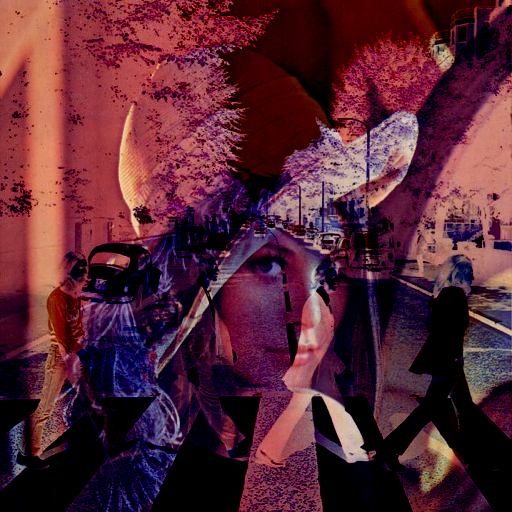
\includegraphics [width=0.25\textwidth]{images/abbey-road-lenna-substract} }
					\caption{Examples de blending}
					\label{fig:blending}
				\end{figure}
		\subsection{Rasterisation}
			La rasterisation consiste à générer une image bitmap à partir du dessin. Cette opération est essentielle puisque l'écrasante
			majorité des dispositifs d'affichage et d'impression ne comprend que des images de ce type. Cette opération doit bien être
			distinguée des opérations de dessin; Effectuer la rasterisation à chaque opération de dessin est l'exception plutôt que la règle.
				
			\subsubsection{Fenêtre de visualisation}
				La pluspart du temps, on ne rasterise pas l'ensemble de la scène à résolution native; On rasterise une zone du dessin
				appelée fenêtre de visualisation. Cette fenêtre peut être de taille variable et représenter l'image à une échelle variable.

			\subsubsection{Accès aléatoire}
				Lorsque l'image est utilisée comme texture dans un moteur de rendu 3D, elle n'est pas accédée d'une manière spatialement
				cohérente. Lorsque la texture est positionnée sur une géométrie 3D, des parties éloignées de la texture peuvent se retrouver
				très proche sur l'objet. De même, lorsque l'objet est lointain, la texture est accédée à faible résolution. Ainsi une même
				texture peut être accédée au cours du même rendu à des endroits différents et à des résolutions différentes. 

			\subsubsection{Modèle colorimétrique et métadonnées}
				La rasterisation d'une image permet de définir la couleur de chaque pixel. Or il existe de nombreuses manière de définir la
				couleur d'un pixel. Premièrement il y a l'espace colorimétrique; Pour afficher sur un écran on utilise le \emph{RGB}. Pour la
				vidéo on utilise le \emph{YUV}. Pour l'impression on utilisera le \emph{CMYK}, ou un système halftone. Certains espaces comme
				le \emph{HSV} ou \emph{CIELab} sont utilisés de manière temporaire afin de faciliter la programation de filtres colorimétriques.
				
				Il y a aussi le choix entre différents niveaux de quantisation : 1bit pour les systèmes halftone; 8bit pour l'affichage 
				à l'écran,  les textures de jeux vidéos; 32 bit flottant permet d'avoir des valeurs de couleurs dépassant les capacité d'affichage
				d'un écran, ce qui est particulièrement intéressant pour l'édition non destructive d'image utilisée en photographie et en 
				effets spéciaux. La précision apportée par une telle profondeur est également indispensable pour le cinéma numérique.  

				Pour le cinéma, les effets spéciaux et les jeux vidéos, on aimera aussi avoir encodé dans chaque pixel des métadonnées 
				sur la géométrie de l'objet physique qu'il représente, telle que sa distance à l'observateur, la normale de la surface
				ou encore l'uid de l'objet auquel il appartient. On est bien loin ici de la notion classique de couleur. 
				
				Les types d'espaces et métadonnées utilisés apparaissent et disparaissent avec les technologies, nécessitant une grande flexibilité
				dans leur gestion. Certains type de frameworks comme les \emph{Éditeurs Nodaux} sont conçus autour de la résolution de ce problème.  

				\begin{figure}[h]
					\centering
					\subfloat[Couleurs vraies]{ \label{fig:render} 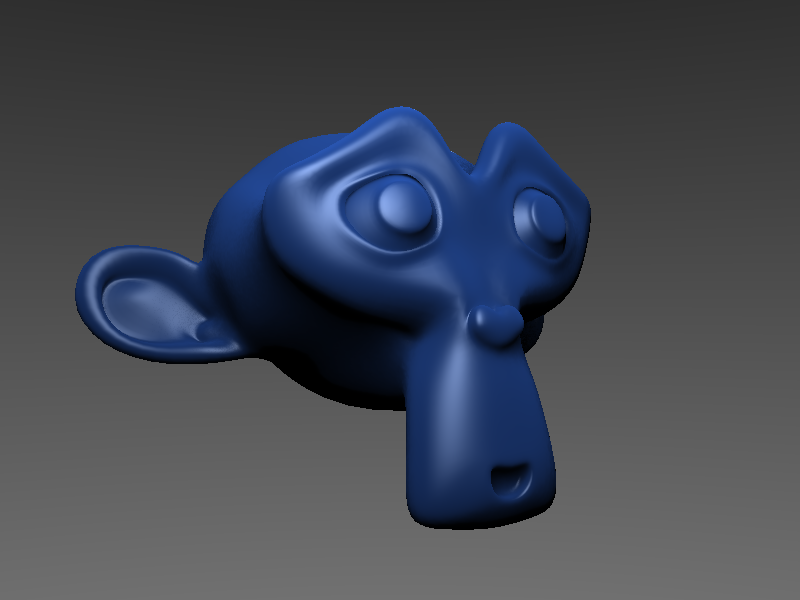
\includegraphics[width=0.25\textwidth]{images/render} }
					\subfloat[Format HSV en fausses couleurs]{ \label{fig:render-hsv} 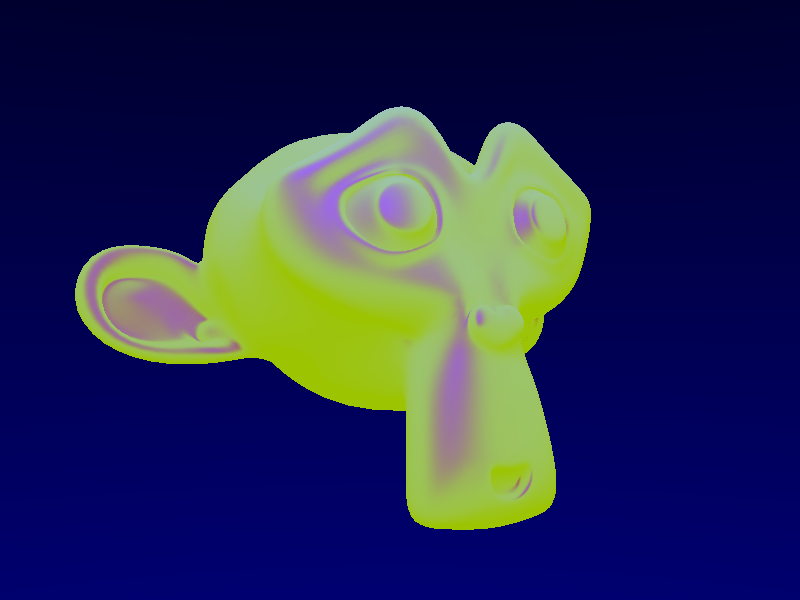
\includegraphics[width=0.25\textwidth]{images/render-hsv} }
					\subfloat[Vecteur normal de la surface]{ \label{fig:render-normal} 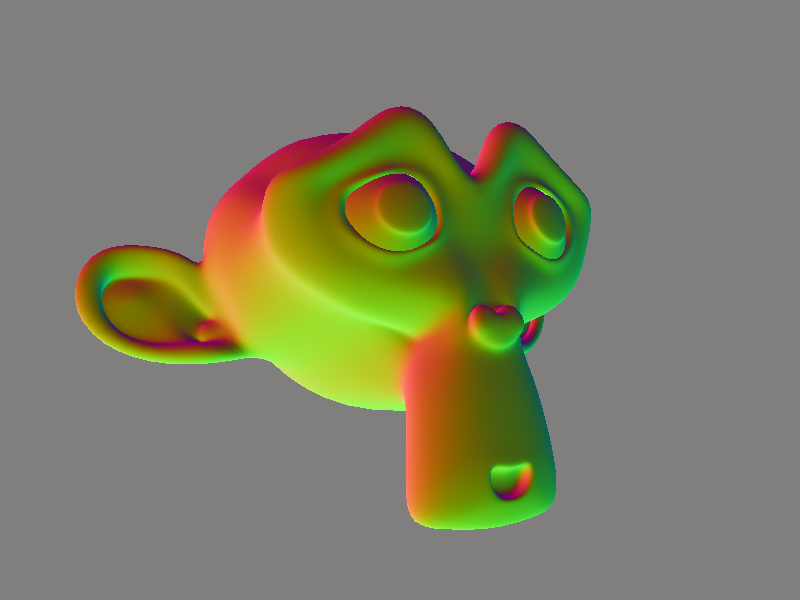
\includegraphics [width=0.25\textwidth]{images/render-normal} }
					\subfloat[Distance à l'observateur]{ \label{fig:render-depth} 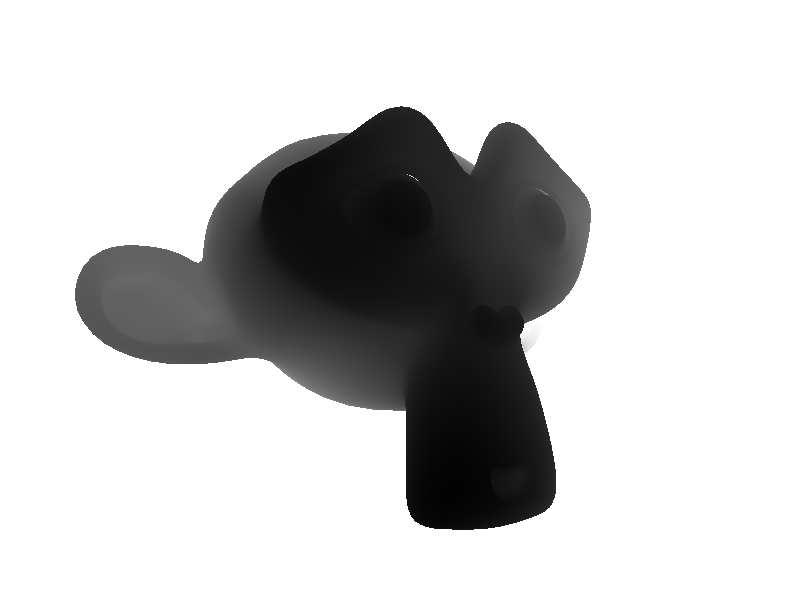
\includegraphics [width=0.25\textwidth]{images/render-depth} }
					\caption{Examples d'espaces colorimétriques et de métadonnées}
					\label{fig:color}
				\end{figure}

		\subsection{Entrée / Sortie sur fichier}
			L'entrée sortie consiste à savoir enregistrer un dessin et le lire depuis un support physique. Différents type de support ont
			différentes caractéristiques de latence, de débit, et de capacité. Certains frameworks peuvent prendre en compte ces caractéristiques afin
			d'améliorer les performances.  
		\subsection{Manipulation d'objets}
			Un framework permet aussi d'interagir avec le dessin en proposant une forme structurée, et de manipuler les opérations
			comme des objets.  
		\subsection{Undo / Redo}
			Un framework a souvent des mécanismes internes permettant une gestion efficace d'annulation et de répétiton des opérations.
		\subsection{Édition non destructive}
			L'édition non destructive, ou édition dynamique consiste à pouvoir modifier une opération après son application.   
		\subsection{Images gigapixels}
			Les images gigapixels sont les images constituées de plus d'un milliard de pixel, qui sont généralement plus grande que la mémoire
			vive disponible. Certains frameworks sont dédiés à la gestion de ce type d'images. 
	\section{Frameworks Bitmaps}
		Les frameworks bitmaps fonctionnent en rasterisant toutes les opérations dès leur application sur l'image. 
		Ce type de framework est particulièrement populaire pour les logiciels de peinture. En effet, les dessins
		de primitives étant appliqués sur l'image, il n'est pas nécessaire de garder en mémoire des structures compliquées
		les mémorisant. De même, les filtres sont particulièrement faciles à implémenter.

		Le rasterising de l'image étant déjà fait à tout moment, les fenêtres de visualisation et l'accès aléatoires sont
		eux aussi efficaces et facile à implémenter. 

		Si les frameworks bitmaps fonctionnent bien pour la peinture, ils sont peu adaptés pour tout le reste:
		\begin{description}
			\item[Modèle colorimétrique et métadonnées:] Les frameworks bitmaps permettent de travailler dans deux espaces colorimétriques,
			celui de travail et celui d'affichage. L'espace de travail est celui que prend en entrée et fournit en sortie toute opération.
			Les données fournies par les opérations sont ensuites converties dans l'espace d'affichage pour être affichées. 

			Il est donc possible de changer d'espace colorimétrique par une opération semblable à un filtre, mais cette opération est destructive,
			impossible par exemple de récupérer la couleur après être passé en noir et blanc. Il est aussi très difficile de gérer des métadonnées.
			Si on dispose à un moment de la couleur et de la normale de chaque pixel, il faut que chaque opération soit programmée pour accepter
			la couleur et la normale, et puisse fournir en sortie une couleur et une normale. Étant donné que les métadonnées utilisées par les
			artistes apparaissent et disparaissent au fil des technologies, ce travail est rarement fait. 

			Ainsi des logiciels comme Gimp ne disposent que de deux espaces de travail, le RGB et le Grayscale. Des logiciels plus avancés comme
			photoshop disposent disposent en outre du CMJN, CIELab, Bichromie, et Multicouches. Cette liste est cependant assez réduite comparée
			à ce qui est utilisé dans des domaines dépassant la photographie et l'impression.
			
			\item[Undo/Redo] Comme chaque opération est directement rasterisée, pour garder trace du résultat des anciennes opérations, il faut
			garder ceux-ci en mémoire. La consommation de mémoire est donc de l'ordre du nombre d'opérations annulables, mais récupérer le résultat
			est instantané.

			\item[Manipulations d'objets] Il est assez difficile de greffer un modèle objet sur un framework bitmap, puisque chaque opération est
			oubliée dès qu'elle est effectuée. 
		\end{description}







	\section{Éditeurs Nodaux}
	\section{Vectoriel}
	\section{Mégatexture}
	\section{Comparaison}
\chapter{Framework Himalaya (20 pages) }
	\section{Structures de données}
		\subsection{Frame}
		\subsection{Image}
		\subsection{Opérations}
		\subsection{États}
	\section{Algorithmes}
		\subsection{Rasterisation}
		\subsection{Dessin}
		\subsection{Sauvegarder l'état}
		\subsection{Charger un état}
		\subsection{Supprimer un état}
		\subsection{Modifier une opération}
	\section{Gestion de la cache}
	\section{Utilisation}
		\subsection{API publique}
		\subsection{Undo / Redo}
		\subsection{Modèle objet par calques}
		\subsection{Modèle objet nodal}
		\subsection{Traits de pinceau}

\chapter{Localité des operations (20 pages)}
	\section{Opérations vectorisées}
		\subsection{Impact sur l'API}
		\subsection{Évaluation des performances}
	\section{Bounding Boxes}
		\subsection{Algorithme Inline}
		\subsection{Algorithme Off-line}
		\subsection{Multi-Niveaux}
		\subsection{Impact sur l'API}
		\subsection{Évaluation des performances}

\chapter{Anti-aliasing (15 pages) }
	\section{Primitive de dessin}
	\section{Problèmes d'échelle}
		\subsection{Oversampling}
	\section{Problèmes de superposition}
	\section{Problèmes de bandes}
	\section{Problème de blending à faible opacité}
	\section{Problème de précision de positionement}
\chapter{Test utilisateurs (10 pages) }
	\section{Procédure}
	\section{Résultats}
	\section{Analyse}
\chapter{Comparaison d'Himalaya aux autres frameworks}
\chapter{Conclusion}
